\documentclass[a4paper,10pt]{article}
\usepackage{fancyhdr}
\usepackage[spanish,activeacute]{babel}
\usepackage{algorithm}
\usepackage{algpseudocode}
\pagestyle{fancy}
\frenchspacing
\usepackage[dvips]{graphicx}
\usepackage[usenames]{color}
\usepackage{colortbl}
\usepackage{amssymb}
\usepackage{caratula}

%Colores
\definecolor{tcA}{gray}{0.90}

%Traducción de instrucciones
\algrenewcommand\algorithmicwhile{\textbf{mientras}}
\algrenewcommand\algorithmicdo{\textbf{hacer}}
\algrenewcommand\algorithmicend{\textbf{fin}}
\algrenewcommand\algorithmicprocedure{\textbf{Procedimiento}}
\algrenewcommand\algorithmicfor{\textbf{para}}
\algrenewcommand\algorithmicif{\textbf{si}}
\algrenewcommand\algorithmicelse{\textbf{sino}}
\algrenewcommand\algorithmicthen{\textbf{entonces}}
\algrenewcommand\algorithmicfunction{\textbf{Funci\'on}}
\algnewcommand\algorithmicto{\textbf{hasta}}

\lhead{\textbf{TP 2}}
\rhead{Capello - Hernandez - Laurito}
\lfoot{Taller de Wiretapping}
\rfoot{\thepage}
\cfoot{ }
\renewcommand{\headrulewidth}{0.6pt}
\renewcommand{\footrulewidth}{0.4pt}
\addtolength{\textwidth}{2cm}
\addtolength{\hoffset}{-0.8cm}
\fancyheadoffset{1cm}
\fancyfootoffset{1cm}

\begin{document}

\materia{Teor'ia de las Comunicaciones}
\submateria{Primer Cuatrimestre de 2013}
\titulo{Taller de Wiretapping}
%\subtitulo{}
\grupo{Grupo:}
\integrante{Mat\'ias Capello}{006/02}{matiascapello@gmail.com}
\integrante{Santiago Hern'andez}{/}{santi-hernandez@hotmail.com}
\integrante{Andr'es Laurito}{/}{andy.laurito@hotmail.com}

\begin{titlepage}
\maketitle
\thispagestyle{empty}
\end{titlepage} 

\pagebreak
\tableofcontents

\pagebreak
\listoffigures

\pagebreak
\thispagestyle{fancy}

\section*{\centering Abstract}
{\em
Meter el resumen al final...
%end italics mode
}
\vspace*{5 mm}

Palabras Clave: 


\section{Introducci'on}
\label{intro1:}

El objetivo de este trabajo pr'actico es abordar algunas nociones de nivel de enlace, poniendo fundamentalmente el foco en el v'inculo con la capa superior y desarrollando un acercamiento anal'itico. El objetivo ser'a analizar de manera interactiva el protocolo \textbf{ARP} y sacar algunas conclusiones de c'omo se comportan los hosts en un segumento de red determinado.

\subsection{ARP - Address Resolution Protocol}

El protocolo \textbf{ARP} tiene un papel clave entre los protocolos de capa de Internet relacionados con el protocolo TCP/IP, ya que permite que se conozca la direcci'on f'isica de una tarjeta de interfaz de red correspondiente a una direcci�n IP. Por eso se llama Protocolo de Resoluci'on de Direcci'on (en ingl'es \textbf{ARP} significa Address Resolution Protocol).

\vspace*{5 mm}
Cada equipo conectado a la red tiene un n'umero de identificaci�n de 48 bits. 'Este es un n'umero 'unico establecido en la f'abrica en el momento de fabricaci'on de la tarjeta. Sin embargo, la comunicaci'on en Internet no utiliza directamente este n'umero (ya que las direcciones de los equipos deber'ian cambiarse cada vez que se cambia la tarjeta de interfaz de red), sino que utiliza una direcci�n l'ogica asignada por un organismo: la direcci'on IP.

\vspace*{5 mm}
Para que las direcciones f'isicas se puedan conectar con las direcciones l'ogicas, el protocolo \textbf{ARP} interroga a los equipos de la red para averiguar sus direcciones f'isicas y luego crea una tabla de b'usqueda entre las direcciones l'ogicas y f'isicas en una memoria cach'e.

\vspace*{5 mm}
Cuando un equipo debe comunicarse con otro, consulta la tabla de b'usqueda. Si la direcci'on requerida no se encuentra en la tabla, el protocolo \textbf{ARP} env'ia una solicitud a la red. Todos los equipos en la red comparan esta direcci'on l'ogica con la suya. Si alguno de ellos se identifica con esta direcci'on, el equipo responder'a al \textbf{ARP}, que almacenar'a el par de direcciones en la tabla de b'usqueda, y, a continuaci'on, podr'a establecerse la comunicaci'on. 

\vspace*{5 mm}
La Figura 1 muestra el formato del paquete \textbf{ARP} para el mapero de direcci'on IP-a-Ethernet. De hecho, \textbf{ARP} puede ser utilizado para muchos otros tipos de mapeos �
las mayores diferencias se dan en los tama\~nos de direcci'on. Adem'as de los OP y las direcciones de capa de enlace de ambos origen y destino, el paquete contiene:

\begin{itemize}
	\item Un campo HardwareType, que especifica el tipo de red f'isica (por ejemplo, Ethernet).
	\item Un campo ProtocolType, que especifica el protocolo de la capa superior (por ejemplo, IP).
	\item Campos HLen (�hardware� address length) y PLen (�protocol� address length), que especifican las longitudes de la direcci'on de capa de enlace y la direcci'on de la capa superior, respectivamente.
	\item Un campo Operation, que especifica si se trata de una solicitud o una respuesta.
	\item Las direcciones de origen y destino del hardware (Ethernet) y protocolo (IP).
\end{itemize}

\begin{figure}[!hbp]
\begin{center}
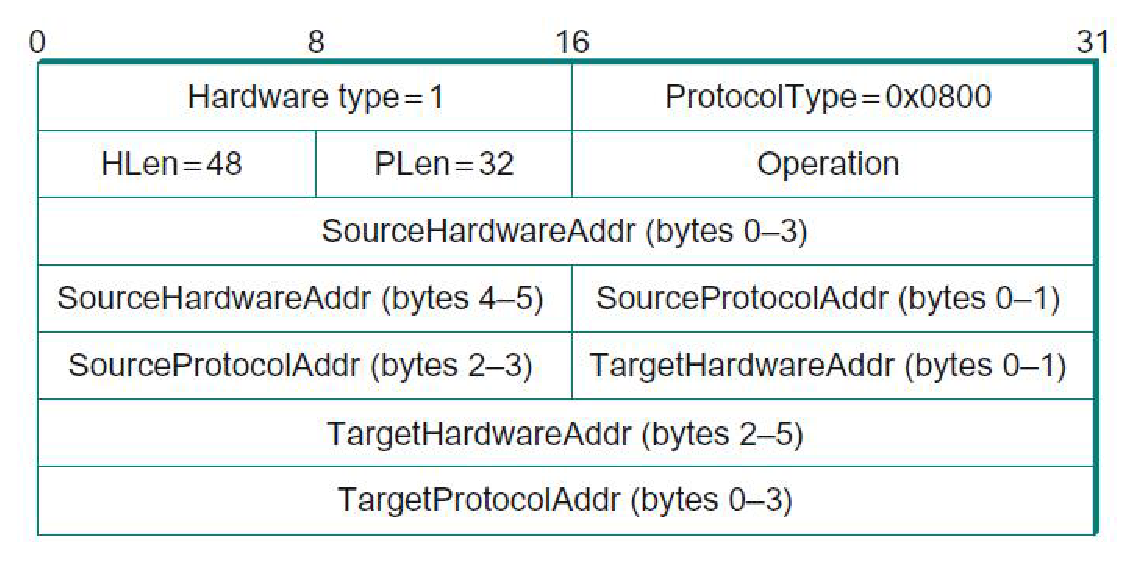
\includegraphics[width=12cm]{figura1.eps}
\end{center}
\caption{Figura 1 - Formato del paquete ARP para el mapeo de direcciones IP a direcciones Ethernet} \label{figura1}
\end{figure}

\subsection{Entrop'ia - Informaci'on}

En el 'ambito de la teor'ia de la informaci'on la entrop'ia, tambi'en llamada entrop'ia de la informaci'on y entrop'ia de Shannon (en honor a Claude E. Shannon), mide la incertidumbre de una fuente de informaci'on.

\vspace*{5 mm}
La entrop'ia tambi'en se puede considerar como la cantidad de informaci'on promedio que contienen los s'imbolos usados. Los s'imbolos con menor probabilidad son los que aportan mayor informaci'on; por ejemplo, si se considera como sistema de s'imbolos a las palabras en un texto, palabras frecuentes como \texttt{que}, \texttt{el}, \texttt{a} aportan poca informaci'on, mientras que palabras menos frecuentes como \texttt{corren}, \texttt{ni\~no}, \texttt{perro} aportan m'as informaci'on. Si de un texto dado borramos un \texttt{que}, seguramente no afectar'a a la comprensi'on y se sobreentender'a, no siendo as'i si borramos la palabra \texttt{ni\~no} del mismo texto original. Cuando todos los s'imbolos son igualmente probables (distribuci'on de probabilidad plana), todos aportan informaci'on relevante y la entrop'ia es m'axima.

\vspace*{5 mm}
El concepto de entrop'ia es usado en termodin'amica, mec'anica estad'istica y teor'ia de la informaci'on. En todos los casos la entrop'ia se concibe como una \textit{medida del desorden} o la \textit{peculiaridad de ciertas combinaciones}. La entrop'ia puede ser considerada como una medida de la incertidumbre y de la informaci'on necesarias para, en cualquier proceso, poder acotar, reducir o eliminar la incertidumbre. Resulta que el concepto de informaci'on y el de entrop'ia est'an ampliamente relacionados entre s'i, aunque se necesitaron a\~nos de desarrollo de la mec'anica estad'istica y de la teor'ia de la informaci'on antes de que esto fuera percibido.

\vspace*{5 mm}
Shannon ofrece una definici'on de entrop'ia que satisface las siguientes afirmaciones:

\begin{itemize}
	\item La medida de informaci'on debe ser proporcional (continua). Es decir, el cambio peque\~no en una de las probabilidades de aparici'on de uno de los elementos de la se\~nal debe cambiar poco la entrop'ia.
	\item Si todos los elementos de la se\~nal son equiprobables a la hora de aparecer, entonces la entrop'ia ser'a m'axima.	
\end{itemize}

\subsubsection{Definici'on Formal}

Supongamos que un fen'omeno (variable aleatoria) tiene un grado de indeterminaci'on inicial igual a k (k estados posibles) y supongamos todos los estados equiprobables, entonces la probabilidad p de que se d'e una de esas combinaciones ser'a 1/k. Podemos representar entonces la expresi�n  $c_{i}$ como:

\vspace*{5 mm}
$c_{i} = log_{2}(k) = log_{2}\left[ 1 \div (1 \div k)\right] = -log_{2}(p)$
\\

Si ahora cada uno de los k estados tiene una probabilidad $p_{i}$, entonces la entrop'ia vendr'a dada por la suma ponderada de la cantidad de informaci'on:

\vspace*{5 mm}
$H = -p_{1}log_{2}(p_{1}) - p_{2}log_{2}(p_{2}) - ... -p_{k}log_{2}(p_{k}) = -\sum^{k}_{i=1} p_{i}log_{2}(p_{i})$
\\

Por lo tanto, la entrop'ia de un mensaje X, denotado por H(X), es el valor medio ponderado de la cantidad de informaci'on de los diversos estados del mensaje:

\vspace*{5 mm}
$H(X) = -\sum_{i} p(x_{i})log_{2}p(x_{i})$
\\

\section{Desarrollo}
\label{desarrollo1:}
\subsection{Primera consigna: Implementaci'on de un cliente ARP}
\label{expli1:}

Se utiliz'o \textit{Scapy} para implementar un script que reciba una direcci'on IP, realice un pedido de su MAC Address y lo devuelva.

La funci'on implementada para resolver esto es \texttt{preguntarMAC}, que recibe una direcci'on IP por par'ametro

Dentro de dicha funci'on se ejecuta lo siguiente:

\vspace*{5 mm}
\texttt{mensajeARP = srp1(Ether(dst="ff:ff:ff:ff:ff:ff")/ARP(pdst=ip),timeout=2)}
\vspace*{5 mm}

Mediante srp1, se env'ia el paquete ARP en broadcast y se acepta solo la primer respuesta (suponemos que solo uno contesta). \texttt{Ether(dst="ff:ff:ff:ff:ff:ff")} es para mandarlo en modo broadcast y \texttt{ARP(pdst=ip)}, la IP de la que le pregunto su MAC Address.

\vspace*{5 mm}
Se prob'o esta funcionalidad con diferentes direcciones de IP, para analizar el resultado obtenido:

\begin{itemize}
	\item direcci'on inexistente: No hay respuesta, se cae por timeout.
	\item direcci'on de la m'aquina origen: ???
	\item direcci'on Broadcast: No hay respuesta, se cae por timeout.
	\item alguna mas???
\end{itemize}

\subsection{Segunda consigna: Capturando tr'afico}
\label{expli1:}

\subsection{Tercera consigna: Gr'aficos y an'alisis}
\label{expli1:}

\section{Resultados}
\label{resultados1:}

\section{An'alisis de resultados}
\label{analisis1:}

\section{Conclusiones}
\label{conclusion1:}

\begin{thebibliography}{99}
\end{thebibliography}

\end{document}

